% COMMON RINGS
\newcommand{\N}{\mathbb{N}}
\newcommand{\R}{\mathbb{R}}
\newcommand{\Z}{\mathbb{Z}}
\newcommand{\T}{\mathbb{T}}
\renewcommand{\S}{\mathbb{S}}

% KNOT THEORETIC

% Crossings and singularities
\newcommand*{\double}{\adjustbox{valign=c}{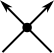
\includegraphics[width=0.05\textwidth]{graphics/glyph_singular_point.pdf}}}
\newcommand*{\poscross}{\adjustbox{valign=c}{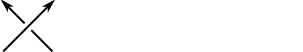
\includegraphics[width=0.05\textwidth]{graphics/glyph_positive_crossing.pdf}}}
\newcommand*{\negcross}{\adjustbox{valign=c}{\includegraphics[width=0.05\textwidth]{graphics/glyph_negative_crossing.pdf}}}
